\documentclass[11pt, a4paper]{jsarticle}
\usepackage{multicol}  % パッケージの追加
\usepackage[dvipdfmx]{graphicx}
\begin{document}
%=============================================================
%=============================================================
\section{Diffraction grating fabrication by two-beam interference}
\subsection*{Purpose}
今回の実験の目的は二光干渉によってフォトクロミックプレートに作られた干渉模様を記録することである.
またフォトクロミックプレートにできた干渉模様によって回折する光について計測し,その干渉模様を理論的に考察する.
\subsection{Diffraction grating fabrication by two-beam interference}
\subsubsection{Procedure}
図\ref{fig:22}のように光学系を製作する.
まず偏光板を光路に挿入して光の強度を下げておく.
偏光された光を50\%のビームスプリッターによってビームを二つに分ける.
分けたビームをそれぞれミラーで反射させてフォトクロミックプレートで一点に集まるように調節する.
この時分けられた光のそれぞれの光路を$Path1=BS - M2 - filter holder$,$Path2=BS - M1 - M3 - filter holder$とする.
光の干渉により回折格子を作りたいのでこのPath1,Path2の光路差がコヒーレント長を上回らないように注意する.
今回の実験での光路長は$Path1=74cm$,$Path2=74cm$であり光路差は0cmとなった.
また二光のなす角$2\theta$が30°を超えないように注意してフィルターホルダー,ミラーの位置を調節する.
今回は$2\theta = 27.7°$とした.
次に偏光板を回し光の強度が強くなるように調節する.
その後フォトクロミックプレートに干渉光を当てることで回折格子をフォトクロミックプレート上に作り出す.
その後フィルターホルダーの後ろに紙をスクリーンとして置き干渉光を観察する.
またPath1,Path2の光を交互に隠すことでスクリーンにどのような干渉スポットが浮かび上がるのかを確認する.

\begin{figure}[htbp]
 \begin{center}
  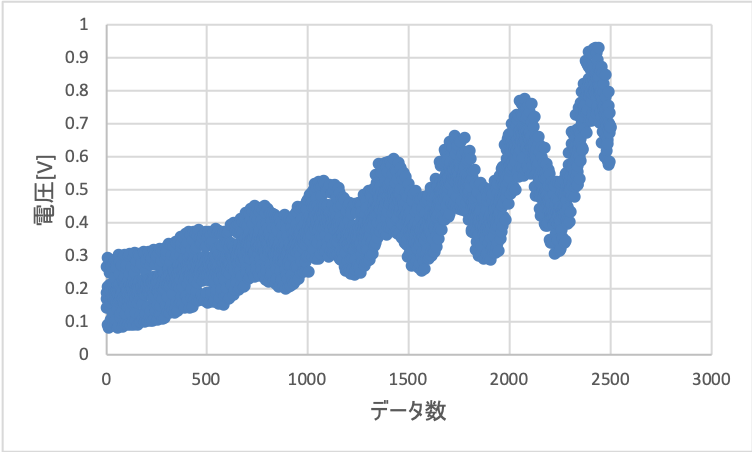
\includegraphics[width=100mm]{fig22.png}
 \end{center}
 \caption{二光干渉による回折格子作成の実験}
 \label{fig:22}
\end{figure}

その次にレーザー光を十分に当てたフォトクロミックプレートを顕微鏡で観察し単位長さあたりに何本の干渉縞が存在しているのかを観察する.

\subsubsection{Result}
偏光板を回転させ光の強度を上げてしばらくフォトクロミックプレートに光を当てると図\ref{fig:28}に示すような干渉スポットがスクリーン上に現れた.
また光路Path1,Path2のどちらを隠しても干渉スッポットは消えることなく存在し続けた.
その後Path2からのビーム光を遮りPath1からの光を用いてスクリーン上の干渉スポットを観察した.
ビーム光の回折格子への入射角は0°,回折角は27.512°であった.
さらに光学顕微鏡で干渉模様を観察すると図\ref{fig:29}に示すような干渉縞が観測された.
干渉縞の本数を数えたところフォトクロミックプレート上には80μmに58本の干渉縞が観察された.
\begin{figure}[htbp]
 \begin{minipage}{0.45\hsize}
  \begin{center}
   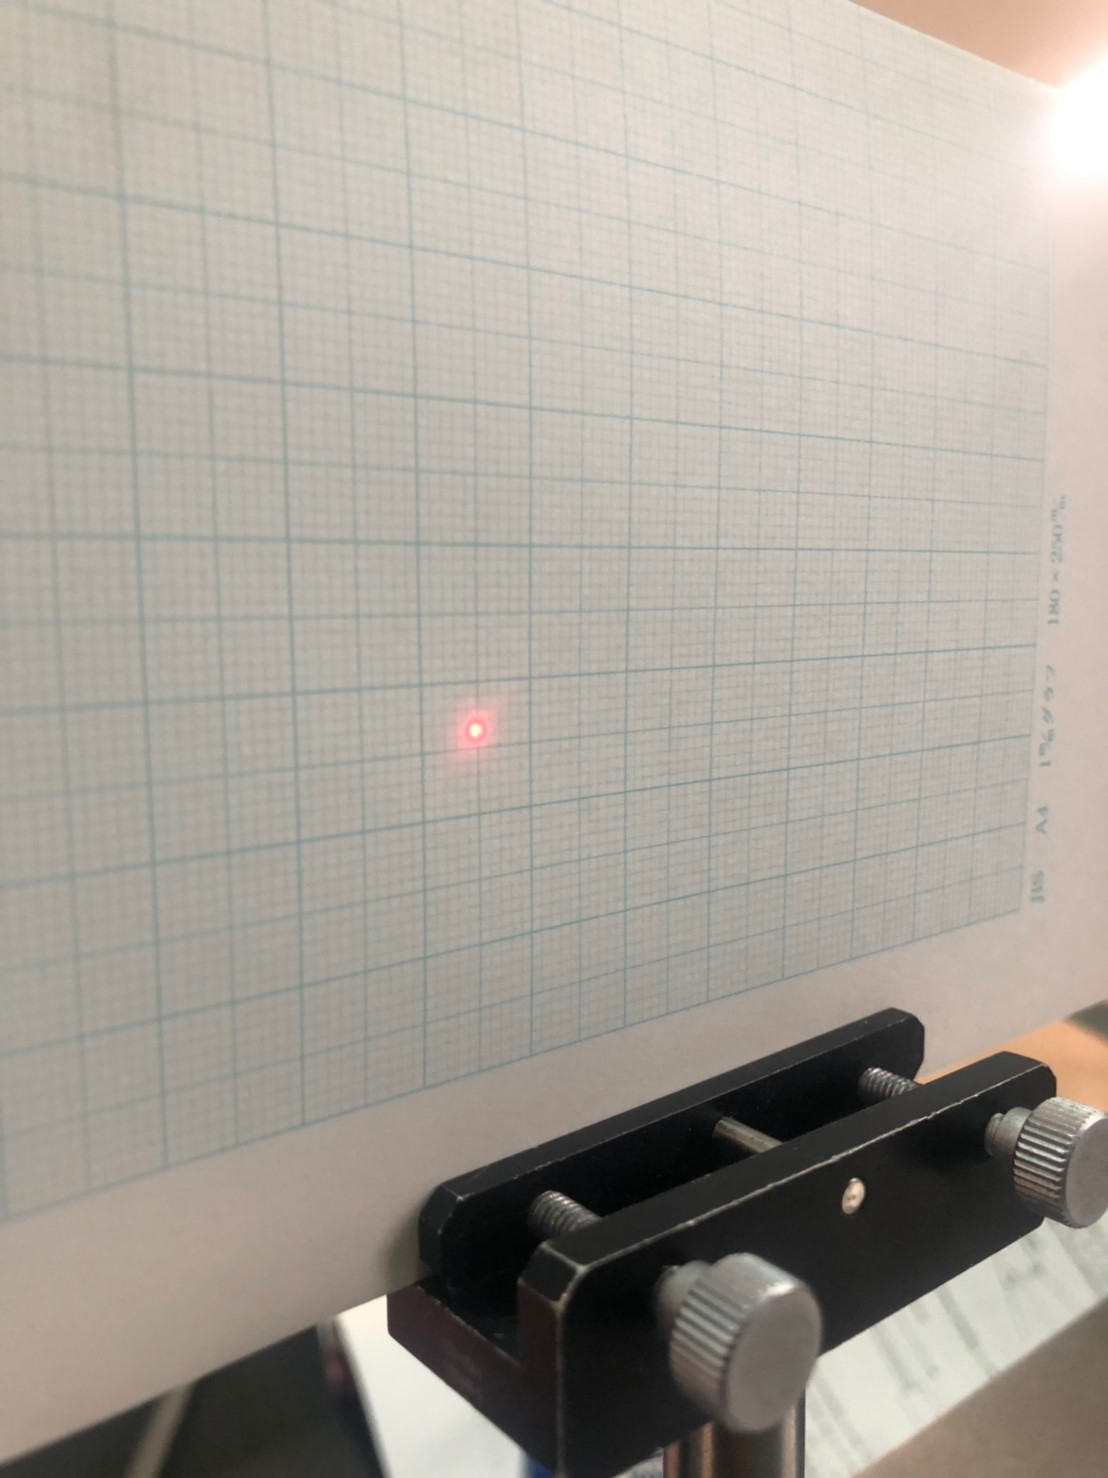
\includegraphics[width=60mm]{fig28.png}
  \end{center}
  \caption{フォトクロミックプレートによってできた干渉縞}
  \label{fig:28}
 \end{minipage}
 \begin{minipage}{0.45\hsize}
  \begin{center}
   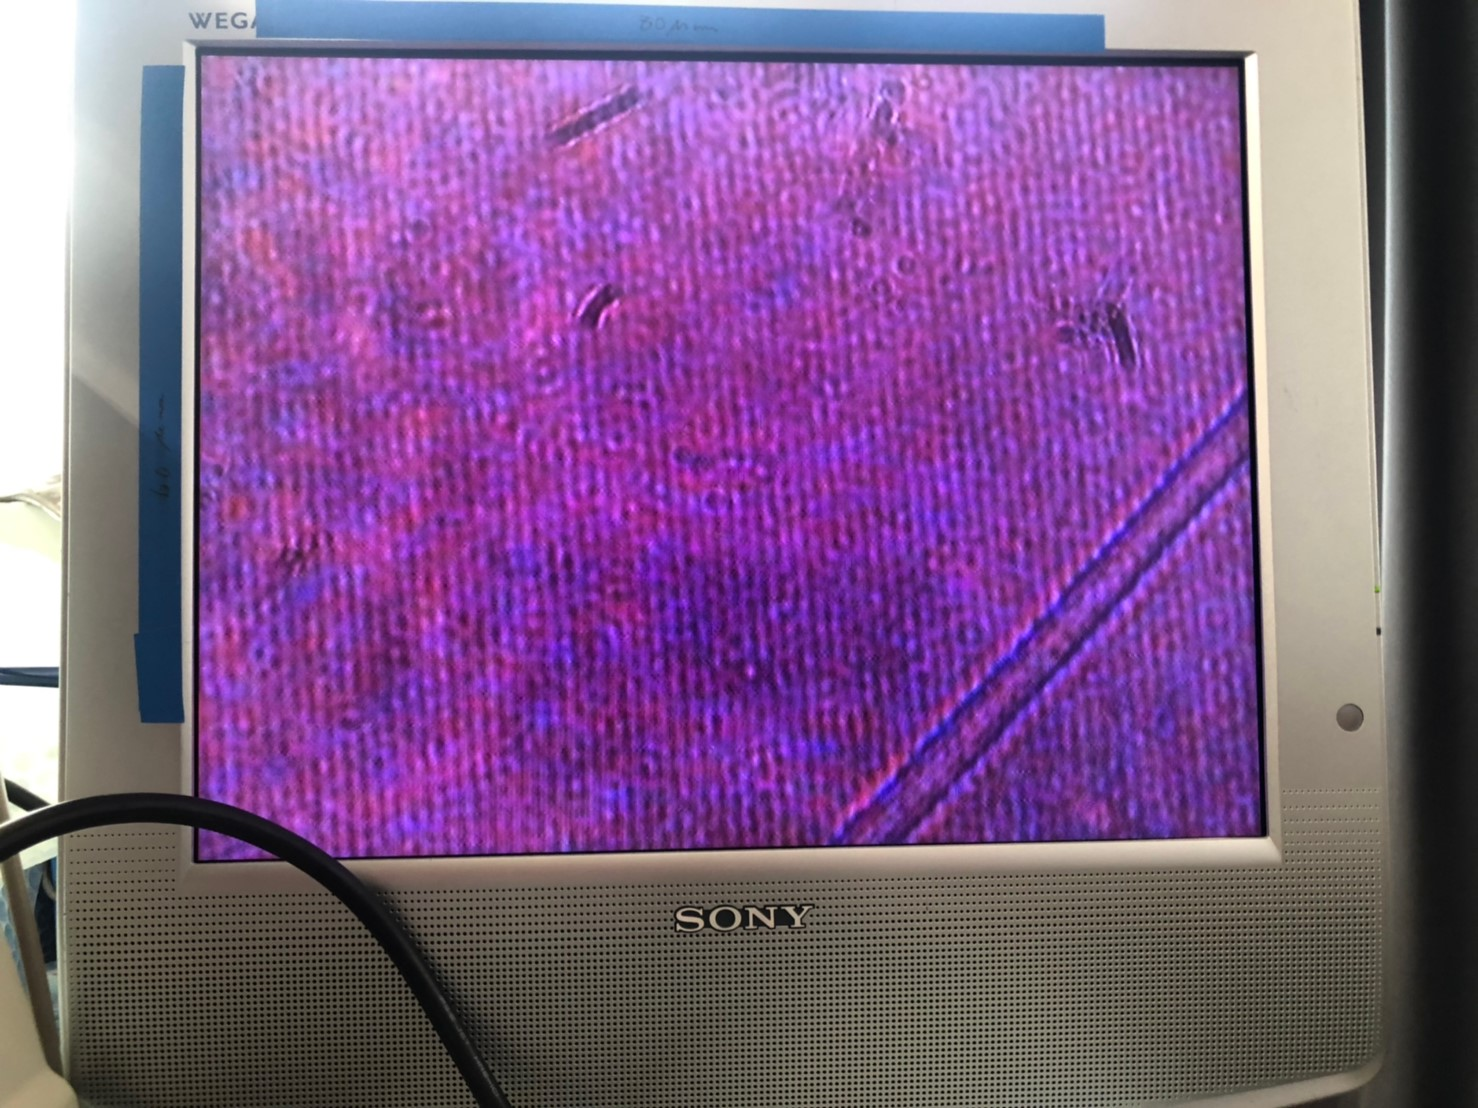
\includegraphics[width=60mm]{fig29.png}
  \end{center}
  \caption{フォトクロミックプレート上の干渉縞}
  \label{fig:29}
 \end{minipage}
\end{figure}

\subsubsection{Discussion}
まずフィルターホルダーの後ろのスクリーンに干渉スポットが観察されたのは,干渉模様がフォトクロミックプレート上にうつされたことにより干渉模様の部分の色がなくなり,フォトクロミックプレートが回折格子の役割を果たしたためだと考えれる.
また,フォトクロミックプレート上に80μmに58本の干渉縞が観察されたことからこの回折格子定数は$d = 1.379μm$であることがわかる.
また回折格子の関係式$\lambda = 2dsin\theta$,さらにHe-Neレーザーの波長($\lambda = 632.8\mu m$)と実験より$2 \theta = 27.7$から格子定数$d =1321.79μm$と計算できる.

以上より回折格子定数の実験値と理論値は概ね一致した.
しかし$\theta$の値が大きかったために回折格子定数が小さくり目測で80μmの中に何本の干渉縞があるのかを観察するのが困難になってしまったために理論値に多少の誤差が生じてしまったことなどが考えられる.

またスクリーン上に映った回折光は一つしか観察されなかったのでm = -1,入射角$\theta_1 = 0°$として回折格子の干渉条件
$dsin\theta_1 - dsin\theta_2 = m\lambda$ の関係式に代入して回折角を求めると,$\theta_2 = 27.316$であり実験で計測した27.512°と近い値となった.
この時回折格子に対して入射角が完全に垂直ではなかったことなどが値が異なった理由として考えられる.
%==========================================================
%==========================================================
\newpage
\end{document}
